\begin{boxE}
 \lr{
 \lstinputlisting[language=Python]{IR5/code/job_4.py}
 }   
\end{boxE}

\begin{figure}
    \centering
    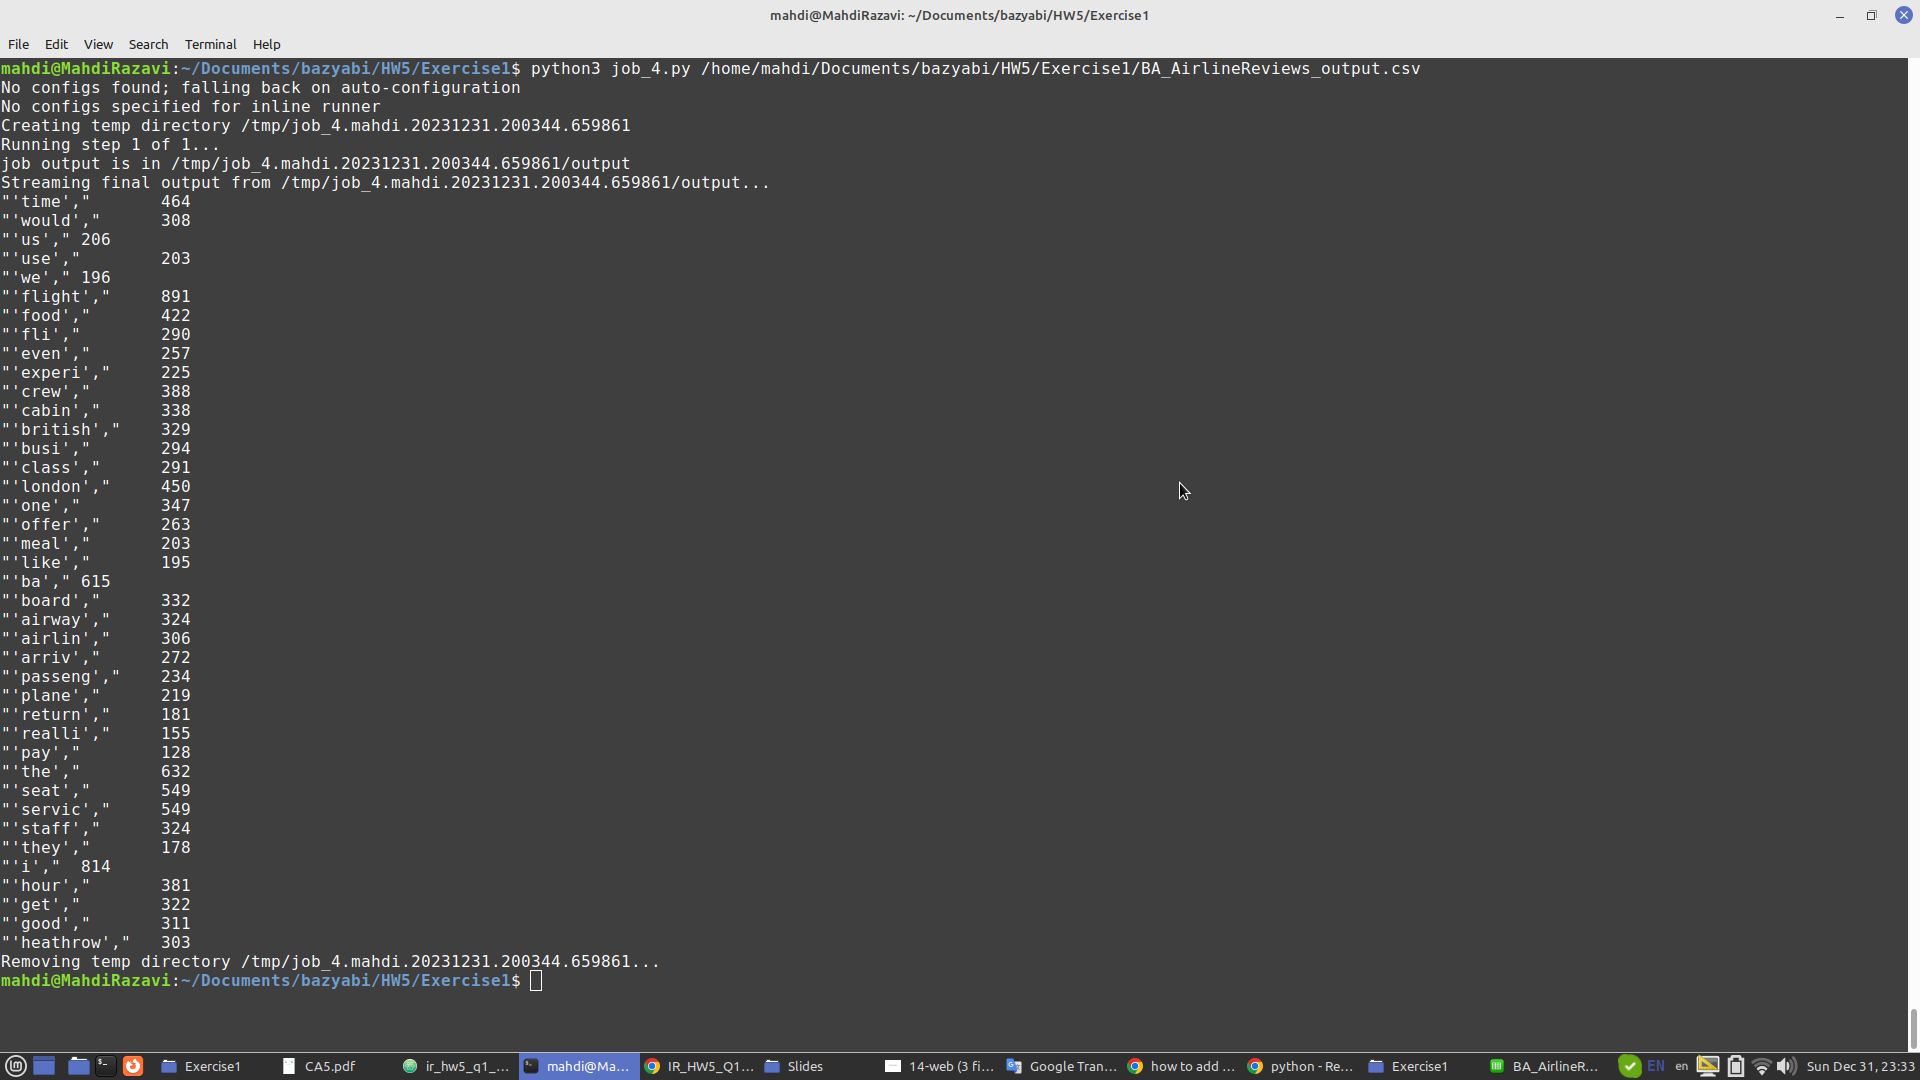
\includegraphics
    [width = 0.9\textwidth]
    {IR5/image/MapReduce_4.png}
    \caption{
    کلماتی که در بیشترین نظرات تایید شده ظاهر شده‌اند.
    }
    \label{fig:enter-label}
\end{figure}

\begin{figure}
    \centering
    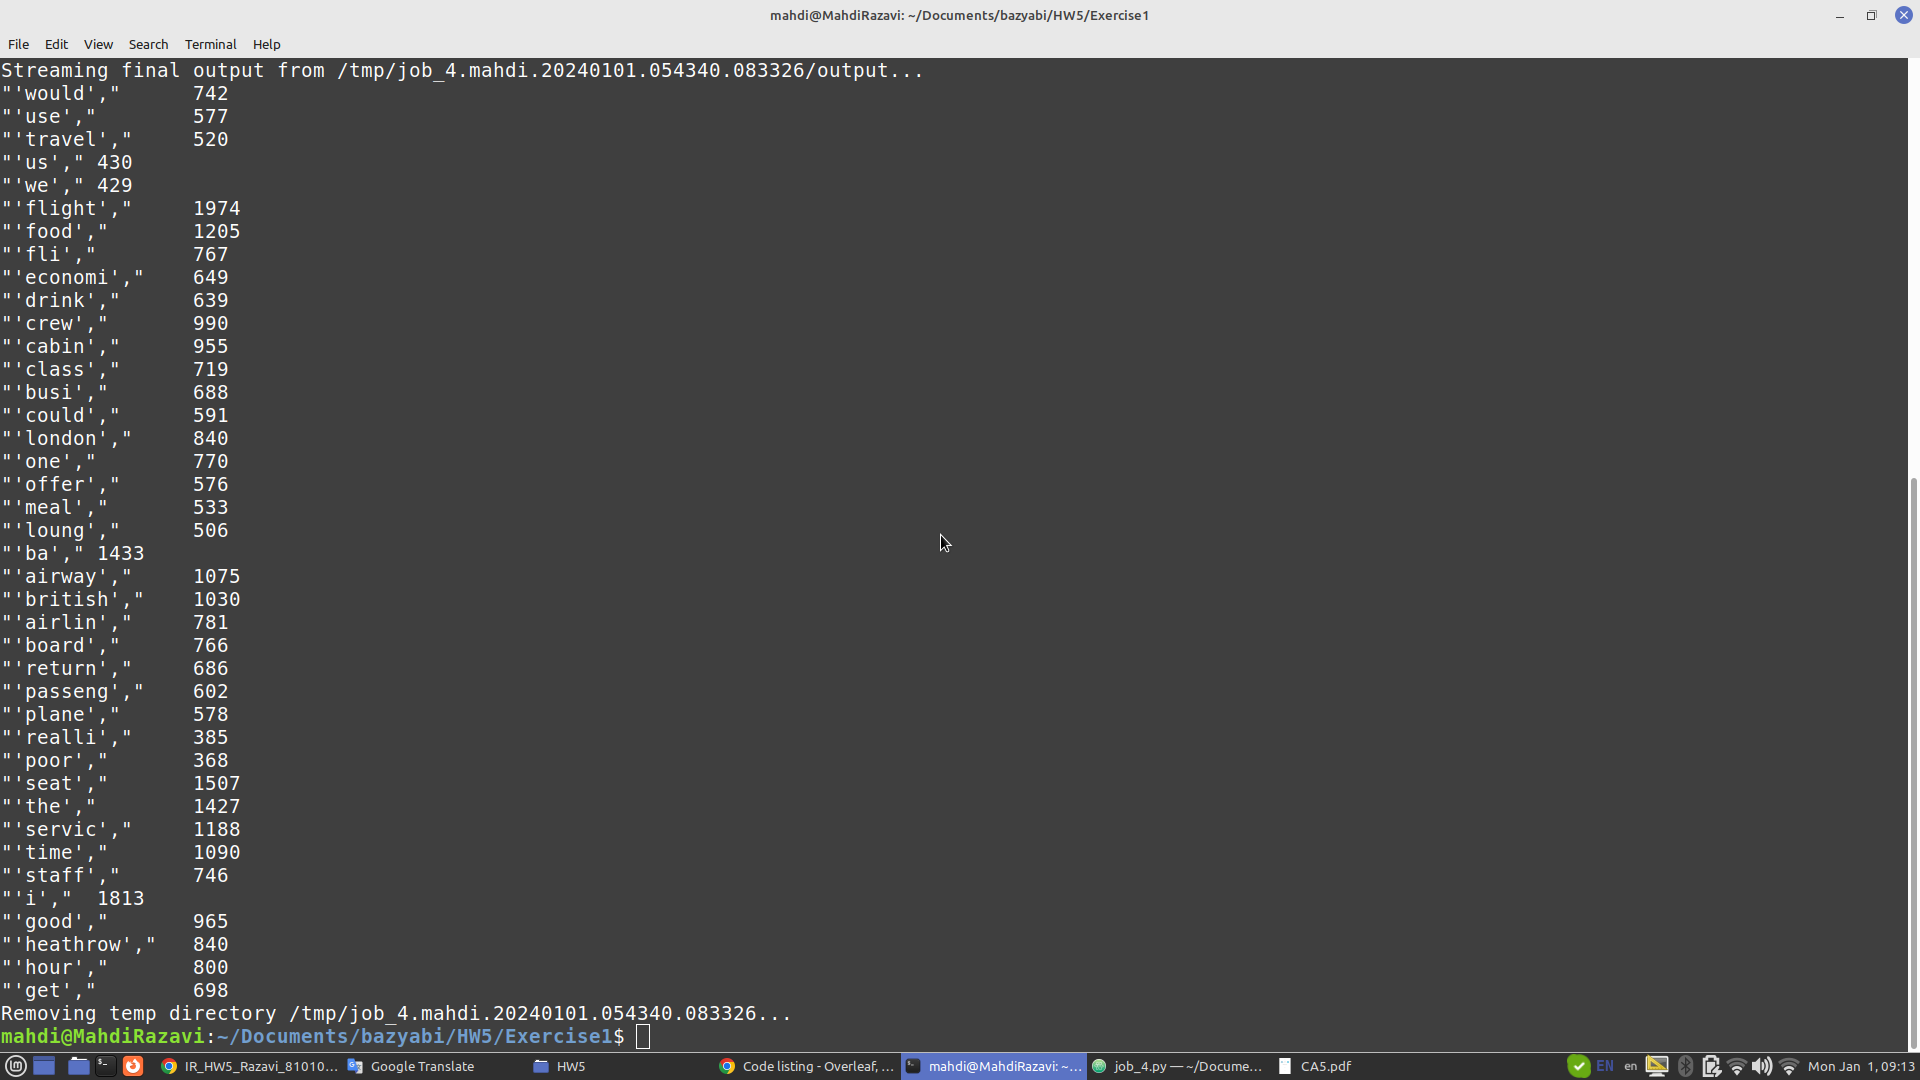
\includegraphics
    [width = 0.9\textwidth]
    {IR5/image/Mr4_False.png}
    \caption{
    کلماتی که در بیشترین نظرات تایید نشده ظاهر شده‌اند.
    }
    \label{fig:enter-label}
\end{figure}

\begin{boxM}
    % توضیحات نوشته شود.
    این گام بسیار شبیه به گام قبل می‌باشد با این تفاوت که در گام 
    \lr{Reducer}
    یک قید دیگر به ازای هر سطر وجود دارد که باید ستون تایید شده یا 
    \lr{True}
    باشد و یا این که 
    \lr{False}
    باشد.
\end{boxM}